% http://tex.stackexchange.com/a/7816/32098
\begin{tikzpicture}[
    title/.style={font=\scriptsize\color{black!75}},
    textlgd/.style={font=\tiny, anchor=west}]
    \node (legende) [title] at (-4.5,-0.41) { Légende };
    \node (region) [below=of legende.west, textlgd, xshift=2mm] { région };
    \draw[] (region.east) -- ++(0.8cm,0cm) node (traitregion) {};
    \node (departement) [below=of region.west, textlgd] { département };
    \draw[dotted] (departement.east) -- ++(0.8cm,0cm) node (traitdepartement) {};
    \node[inner sep=0pt,outer sep=2pt,draw=black!50,fit={(legende) (region) (departement) (traitregion) (traitdepartement) }] (lgdbox) {};
    \node[align=center,below] at (lgdbox.south) {Métamodèle};

    \pic[local bounding box=carte] (carte) at (0, 0) {france={scale 0.15}};
    \node[align=center,below] at (carte.south) {Modèle};

    \node[inner sep=2pt] (photo) at (6,-1.4) {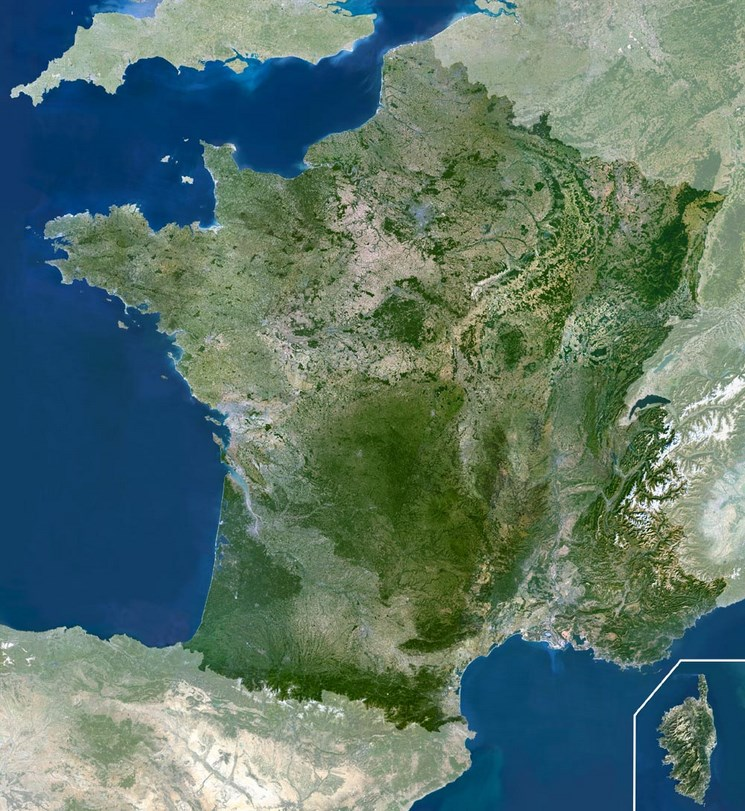
\includegraphics[scale=0.09]{figures/lib/france_satellite.jpg}};
    \node[align=center,below] at (photo.south) {Système modélisé};

    % fleches
    \draw[->] (carte) -- (photo.west) node[midway,above] {Représente} node[midway,below]{$\mu$};
    \draw[<-] (lgdbox)   -- (carte.west) node[midway,above] {ConformeÀ}  node[midway,below]{$\chi$};
\end{tikzpicture}
